L'interfaccia utente del nostro elaborato è un prototipo di ciò che sarà effettivamente la piattaforma.\\
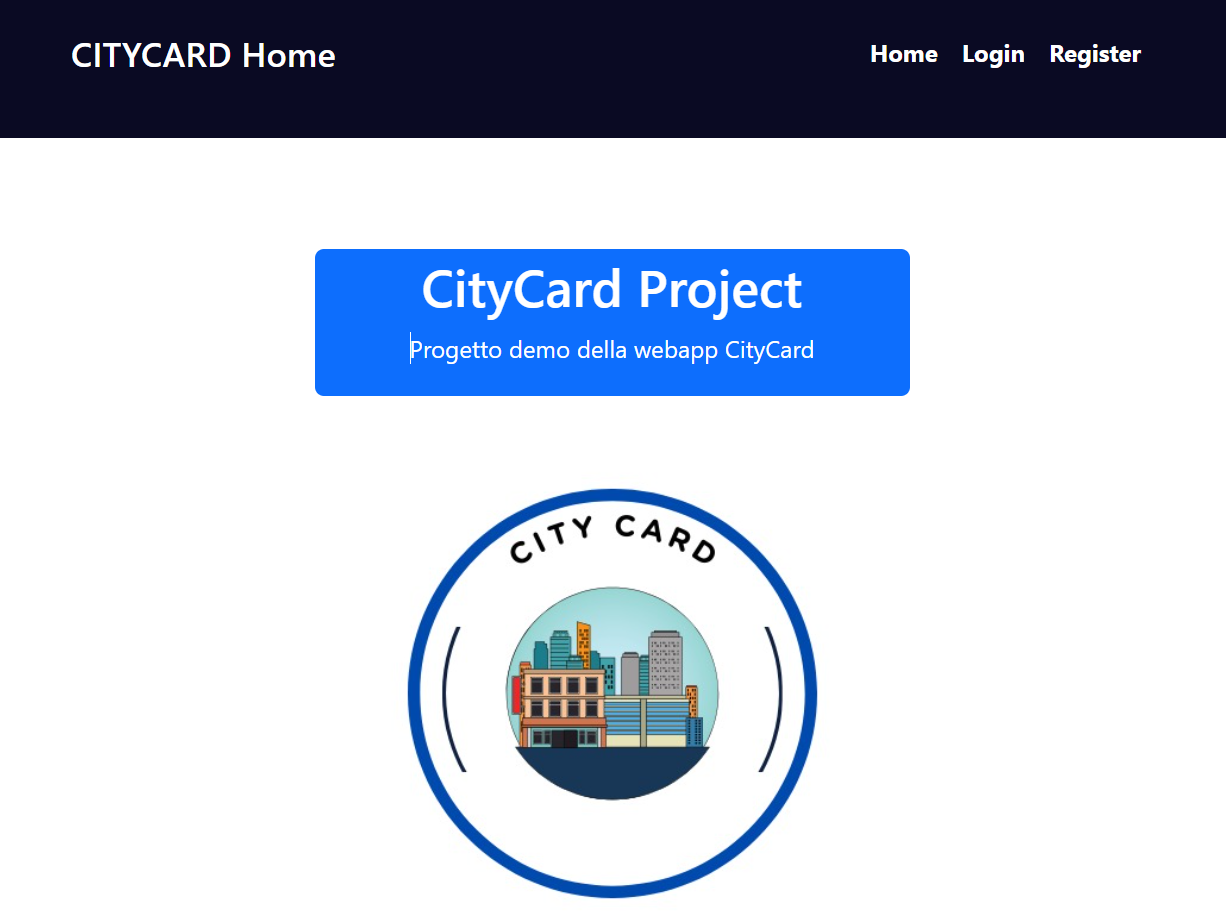
\includegraphics[width=0.95\columnwidth]{home.png}\\
L'applicazione è stata realizzata appoggiandosi al framework Node.js. 
I linguaggi utilizzati sono JavaScript per la parte logica e back end, dei fogli di stile CSS e di Bootstrap per quanto concerne l'aspetto grafico. 
Il database è in locale e il DBMS usato è mySQL.
Per la comunicazione con il database è stato utilizzato Express per creare una REST API.\\
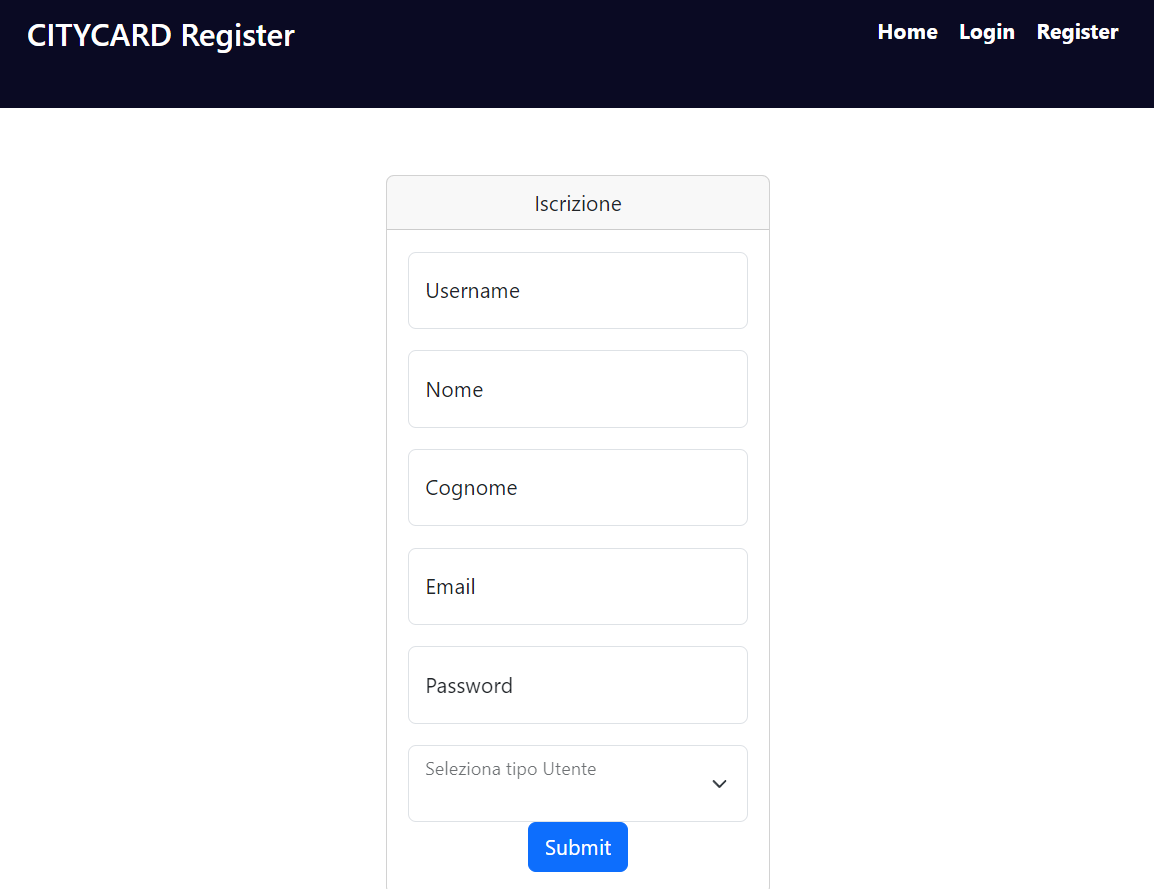
\includegraphics[width=0.95\columnwidth]{register.png}\\
Nella schermata iniziale di registrazione sarà possibile, oltre ai dati principali come username e password, il proprio ruolo all'interno del sito.\\
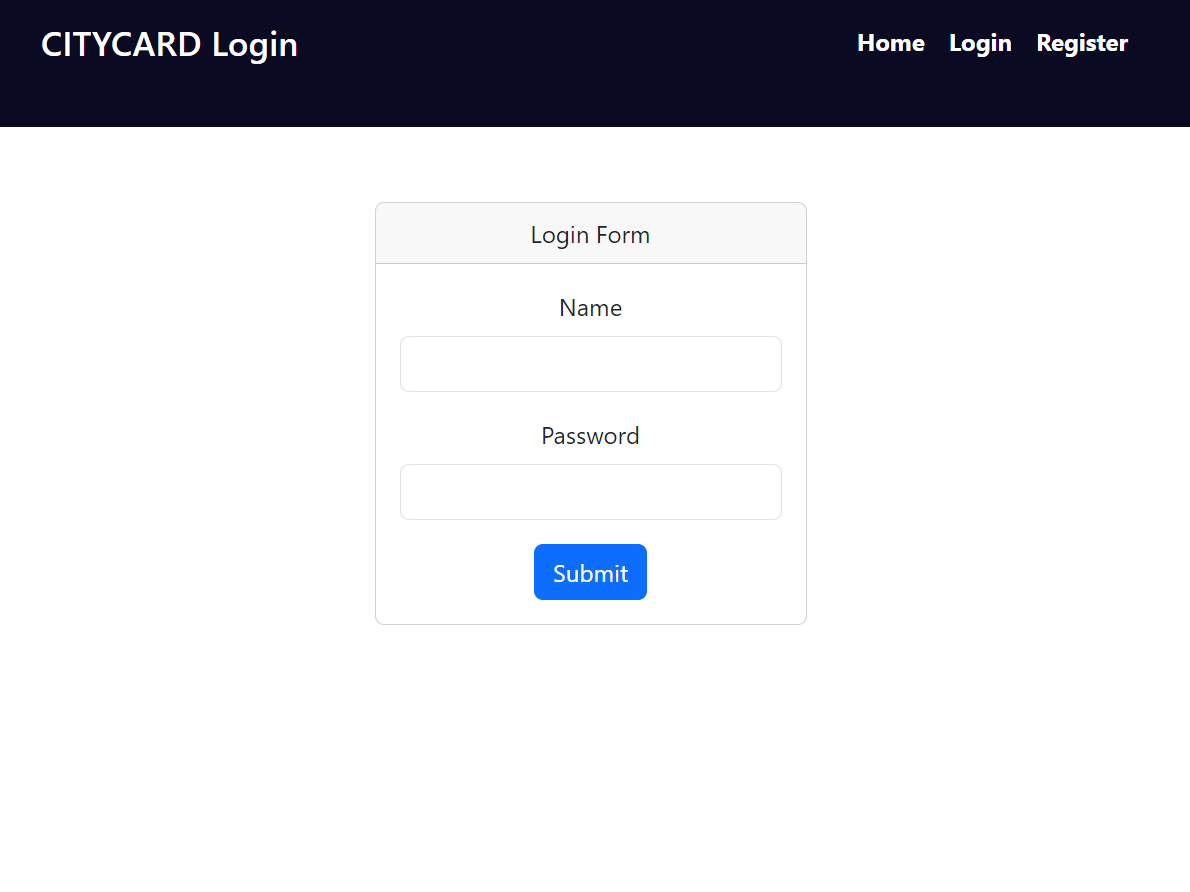
\includegraphics[width=0.95\columnwidth]{login.png}\\
Una volta registrato l'utente si potrà loggare nell'applicazione accedendo alla parte dedicata al proprio tipo utente.\\
\vfill
Ci si deve occupare di gestire tre tipologie di utenti: gli amministratori, i fornitori e i clienti.
Passiamo ora ad esaminare questo tipo di interfacce e le diverse funzioni da esse offerte.